\documentclass [a4paper,11pt] {report}
\usepackage{graphicx}
\usepackage{pdfpages}
\usepackage{fancybox}
\usepackage[francais]{babel}
\usepackage[utf8]{inputenc}
\usepackage[T1]{fontenc}
\usepackage{amsmath,amsfonts,amssymb}
\usepackage{fancyhdr}
\usepackage{stackrel}
\usepackage{xspace}
\usepackage{url}
\usepackage{titling}
\newcommand{\dsp}{\displaystyle}

\setlength{\parindent}{0pt}
\setlength{\parskip}{1ex}
\setlength{\textwidth}{17cm}
\setlength{\textheight}{24cm}
\setlength{\oddsidemargin}{-.7cm}
\setlength{\evensidemargin}{-.7cm}
\setlength{\topmargin}{-.5in}


%%%%%%
% Pour mise-en-forme des fichiers Ada
%
% voir exemple en fin de ce fichier.
%
% ATTENTION, requiert encoding utf-8 (voir 2ième "\lstset" ci-dessous)
 
\usepackage{listings}
\lstset{
  morekeywords={abort,abs,accept,access,all,and,array,at,begin,body,
      case,constant,declare,delay,delta,digits,do,else,elsif,end,entry,
      exception,exit,for,function,generic,goto,if,in,is,limited,loop,
      mod,new,not,null,of,or,others,out,package,pragma,private,
      procedure,raise,range,record,rem,renames,return,reverse,select,
      separate,subtype,task,terminate,then,type,use,when,while,with,
      xor,abstract,aliased,protected,requeue,tagged,until},
  sensitive=f,
  morecomment=[l]--,
  morestring=[d]",
  showstringspaces=false,
  basicstyle=\small\ttfamily,
  keywordstyle=\bf\small,
  commentstyle=\itshape,
  stringstyle=\sf,
  extendedchars=true,
  columns=[c]fixed
}

% CI-DESSOUS: conversion des caractères accentués UTF-8 
% en caractères TeX dans les listings...
\lstset{
  literate=%
  {À}{{\`A}}1 {Â}{{\^A}}1 {Ç}{{\c{C}}}1%
  {à}{{\`a}}1 {â}{{\^a}}1 {ç}{{\c{c}}}1%
  {É}{{\'E}}1 {È}{{\`E}}1 {Ê}{{\^E}}1 {Ë}{{\"E}}1% 
  {é}{{\'e}}1 {è}{{\`e}}1 {ê}{{\^e}}1 {ë}{{\"e}}1%
  {Ï}{{\"I}}1 {Î}{{\^I}}1 {Ô}{{\^O}}1%
  {ï}{{\"i}}1 {î}{{\^i}}1 {ô}{{\^o}}1%
  {Ù}{{\`U}}1 {Û}{{\^U}}1 {Ü}{{\"U}}1%
  {ù}{{\`u}}1 {û}{{\^u}}1 {ü}{{\"u}}1%
}


\predate{
\begin{center}
}
\postdate{
\\
\vspace{1.5cm}

\includegraphics[scale=0.7]{imag.png}
\end{center}}


\title {{ {\huge Compte rendu du projet}} \\
``{\em Files de priorité, Arbres de Huffman}'' }

\author {Equipe 82 \\
\\
GOUTTEFARDE Léo \\ PIERUCCI Dimitri}
\date{Jeudi 14 Mai 2015}
% \date{Vendredi 1 Mai 2015\endgraf\bigskip
% Equipe NN}

\lhead{Projet d'Algorithmique 2}
\rhead{Compte rendu}

\begin{document}
\pagestyle{fancy}
\maketitle

\begin{center}
\section* {Introduction }
\end{center}

Nous avons traité l'ensemble du sujet, ainsi que l'optimisation de \lstinline!Decodage_Code! et des fonctions de \lstinline!Compression! / \lstinline!Decompression! par l'encodage des arbres de Huffman directement dans le fichier, au lieu d'y laisser la table des fréquences intégrale.

L'exécutable compresse et décompresse sans problème les fichiers texte, et les libérations mémoire sont bien implémentées donc il n'y a pas de memory leak.

L'archive contient l'ensemble du code source au sein du dossier \textit{src}, ainsi que les différents fichiers texte testés dans le dossiers \textit{src/tests}, contenant pour chaque test le fichier \textit{.txt} d'origine, le \textit{.huff} compressé, le \textit{.txt} décompressé, et enfin l'arbre de Huffman correspondant en \textit{dot} et \textit{png}.

Le fichier Makefile du dossier \textit{src} permet quant à lui de tester facilement le programme, on peut notamment changer le nom du test à effectuer (variable \lstinline!NOM!).

La commande \lstinline!make! compile le programme, \lstinline!make run! encode puis décode le test indiqué après compilation, et enfin \lstinline!make dot! exécute \lstinline!make run! puis affiche l'arbre \textit{dot} obtenu.


$\newline$
\section* {1\hspace{5mm}Choix d'implémentation }

Pour l'implémentation des files de priorité, nous avons introduit quelques nouvelles structures :

\begin{lstlisting}

type Element is record
    P : Priorite;
    D : Donnee;
end record;

type Tableau is array (integer range <>) of Element;

type File_Interne (Taille_Max : Positive) is record
    Tas : Tableau(1 .. Taille_Max);
    Taille : Natural := 0;
end record;

\end{lstlisting}
$\newline$
Nous avons ainsi simplement défini le type \lstinline!File_Interne! comme discriminé par la taille maximale de la liste, permettant d'allouer un tableau de taille correspondante pour le \lstinline!Tas!.

Nous avons également un champ \lstinline!Taille! qui permet de savoir combien d'éléments sont réellement contenus, et finalement le type \lstinline!Element! correspond au contenu des cases du \lstinline!Tas!, et se compose donc d'un champ priorité et d'un champ donnée.





\section* {2\hspace{5mm}Démarche de validation }

Pour la démarche de validation fonctionnelle, nous avons d'abord testé nos files de priorité à l'aide du fichier \textit{test\_file.adb}.

Puis, pour corriger notre code de génération de l'arbre de Huffman et donc des codes optimaux, nous avons principalement réutilisé la fonction de génération d'arbre \textit{dot} pour facilement visualiser les problèmes de l'arbre \textit{png} généré. Pour ces tests, nous avons repris l'exemple de construction du sujet avec le mot \textit{``hello''}, au sein du fichier de test \textit{src/tests/test0.txt}.

\newpage

Finalement pour résoudre les problèmes restants après l'optimisation du code de \lstinline!Compression! / \lstinline!Decompression! par encodage de l'arbre de Huffman, nous avons réutilisé le premier exemple du sujet de la chaîne \textit{``acbeceea''}, à l'aide du fichier de test \textit{src/tests/test1.txt} (Figure 1).

\begin{figure}[ht]
\begin{center}
% \centering
  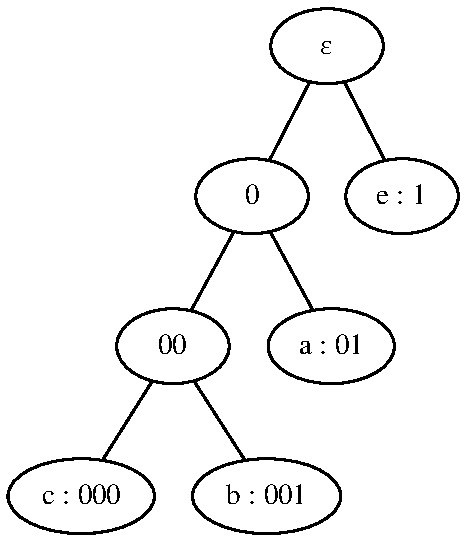
\includegraphics[scale=0.75]{test1.pdf}
 \caption{Arbre de Huffman de \textit{``acbeceea''}}
\end{center}
\end{figure}

Nous avons ainsi facilement pu vérifier la bonne fonctionnalité du code, et finalement corrigé une erreur restante en remarquant une simple inversion des variables de \lstinline!Stream! lors du décodage, qui était à l'origine de notre problème peu complexe au final.


\section* {3\hspace{5mm}Tests de performance }

\subsection* {3.1\hspace{3mm} Gains / pertes d'espace après compression}

Pour évaluer les gains et pertes d'espace après compression, nous avons utilisé plusieurs fichiers de test :

\begin{enumerate}

\item%[$\bullet$]
\textit{src/tests/test0.txt} : mot \textit{``hello''}

\item%[$\bullet$]
\textit{src/tests/test1.txt} : chaîne \textit{``acbeceea''}

\item%[$\bullet$]
\textit{src/tests/test2.txt} : \textit{Lorem Ipsum} classique de 3 paragraphes

\item%[$\bullet$]
\textit{src/tests/test3.txt} : \textit{Lorem Ipsum} aléatoire de 10 paragraphes

\item%[$\bullet$]
\textit{src/tests/test4.txt} : \textit{Lorem Ipsum} aléatoire de 20 paragraphes

\end{enumerate}
\vspace{0.5cm}

Ci-dessous les tailles avant / après compression :
%\hspace{-3.3cm}
\begin{center}
 % \centering
\begin{tabular}{|c|c|c|c|c|c|}
 \hline
Fichier & test0.txt & test1.txt & test2.txt & test3.txt & test4.txt\\
 \hline
Non compressé & 5 o & 8 o & 2 Ko & 3.4 Ko & 7 Ko\\
Compressé & 11 o & 11 o & 1.1 Ko & 1.8 Ko & 3.7 Ko\\
 \hline
\end{tabular}
\end{center}

\newpage

A l'issue de ces tests, on remarque que pour les fichiers relativement petits comme \textit{``hello''} et \textit{``acbeceea''} (deux premiers tests), il y a une légère augmentation de la taille. On aurait pu réduire leur taille de 4 octets en retirant le nombre total de caractères écrit en tête de fichier, cependant nous l'avons gardé car c'est aussi un moyen de simplifier la décompression et de vérifier la taille du contenu décompressé.

En revanche, les \textit{Lorem Ipsum} bénéficient bien d'un gain en espace intéressant, avec une réduction de quasimment 50 \%.

Notre programme de compression par encodage de l'arbre de Huffman en tête de fichier est donc assez puissant.


\subsection* {3.2\hspace{3mm} Vitesse d'exécution}

Les vitesses d'exécution du programme mesurées en moyenne (sans export de l'arbre \textit{dot}) pour les différents tests sont les suivantes :
%\hspace{-3.3cm}
\begin{center}
 % \centering
\begin{tabular}{|c|c|c|c|c|c|}
 \hline
Fichier & test0.txt & test1.txt & test2.txt & test3.txt & test4.txt\\
 \hline
Compression & 3 ms & 3 ms & 5 ms & 5 ms & 8 ms\\
Décompression & 3 ms & 3 ms & 3 ms & 3 ms & 5 ms\\
 \hline
\end{tabular}
\end{center}
\vspace{0.25cm}

On observe que pour les deux premiers tests, la compression et la décompression prennent autant de temps, soit trois millisecondes. C'est probablement une approximation de la borne inférieure de la durée minimale du programme, et vu que les deux textes sont courts la compression et la décompression durent quasimment autant de temps.

Pour les Lorem Ipsum de taille croissante en revanche (trois derniers tests), la vitesse de compression devient un peu plus longue que celle de décompression, jusqu'à 8 ms de compression et 5 ms de décompression pour le Lorem Ipsum de 20 paragraphes contre 5 ms de compression et 3 ms de décompression pour celui de 3 paragraphes.

C'est normal puisque la compression nécessite l'analyse fréquentielle des caractères puis la construction de l'arbre de Huffman, tandis que pour la décompression il suffit d'utiliser l'arbre du fichier compressé.

Ce programme de compression est donc relativement performant d'après les tests effectués.


\end{document}


